% !TEX encoding = UTF-8 Unicode 
% !TEX root = praca.tex

\subsection{Research scenario 3 results analysis}

The following figures illustrate the aggregated results from the experiments conducted within Research scenario 3 described in Chapter \ref{chap:research_scenarios}.

\begin{figure}[H]
    \begin{minipage}{.48\textwidth}
        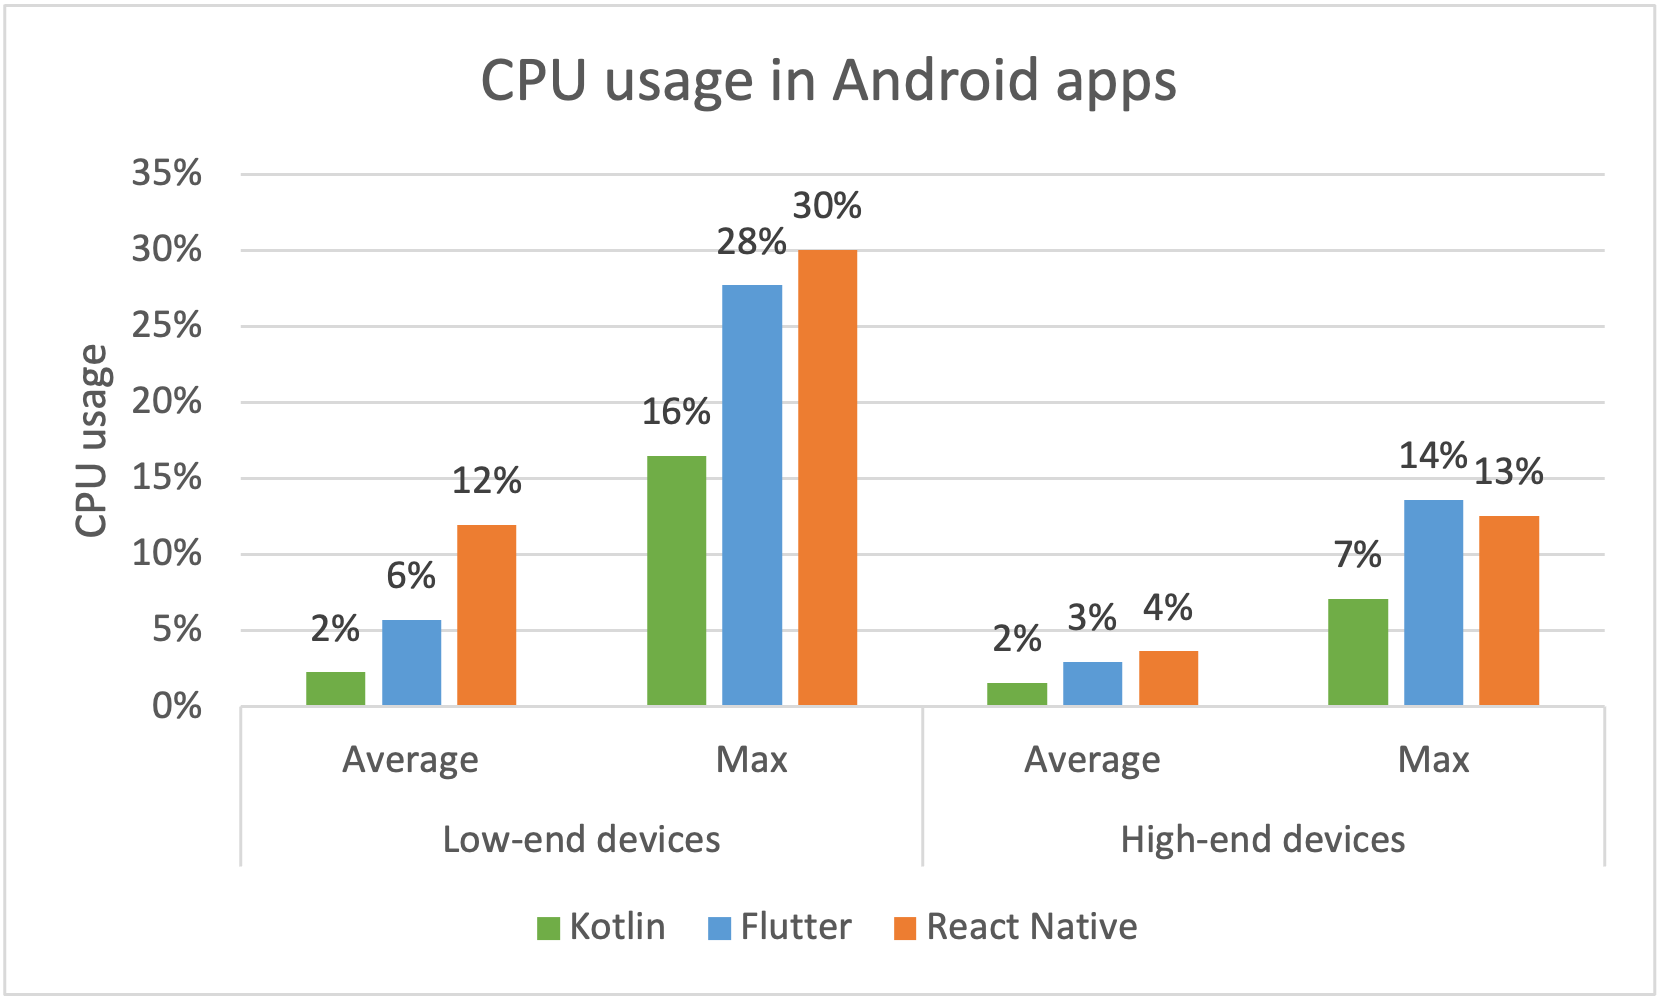
\includegraphics[width=\textwidth]{img/scenario3_cpu_android}
        \caption{Research scenario 3: CPU usage in Android apps (Source: Own work)}
        \label{fig:s3_cpu_android}
    \end{minipage}
    \hfill
    \begin{minipage}{.48\textwidth}
        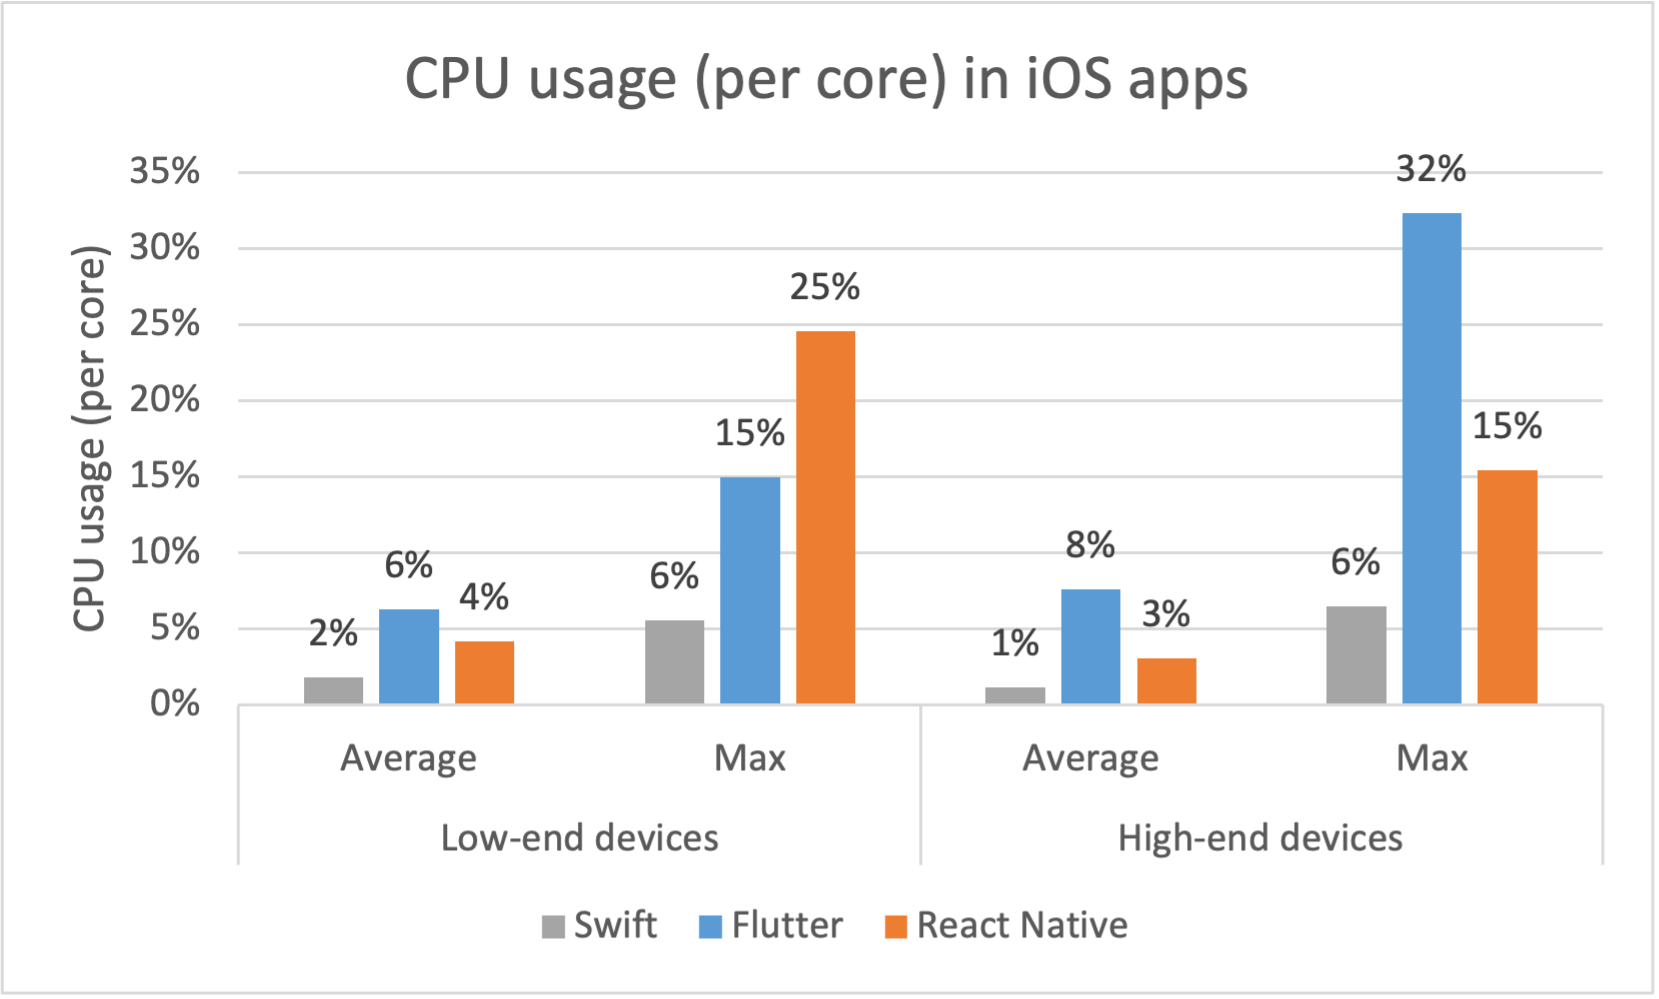
\includegraphics[width=\textwidth]{img/scenario3_cpu_ios}
        \caption{Research scenario 3: CPU usage in iOS apps (Source: Own work)}
        \label{fig:s3_cpu_ios}
    \end{minipage}
\end{figure}

Figures \ref{fig:s3_cpu_android} and \ref{fig:s3_cpu_ios} show the comparison of CPU usage among Android and iOS apps developed with Kotlin, Swift, Flutter, and React Native. On low-end and high-end Android devices, Kotlin apps provide the best performance at 2\% CPU load, followed by Flutter apps at 3--6\% and finally React Native apps at 4-12\%. When it comes to maximums reached, Flutter and React Native are again outperformed by Kotlin, but the values themselves are still relatively low. In the case of iOS, Swift apps show the lowest CPU load as well as no spikes on both low-end and high-end devices. React Native apps demonstrate slightly lower CPU usage than Flutter apps, although they experience higher spikes on low-end devices.

\begin{figure}[H]
    \centering
    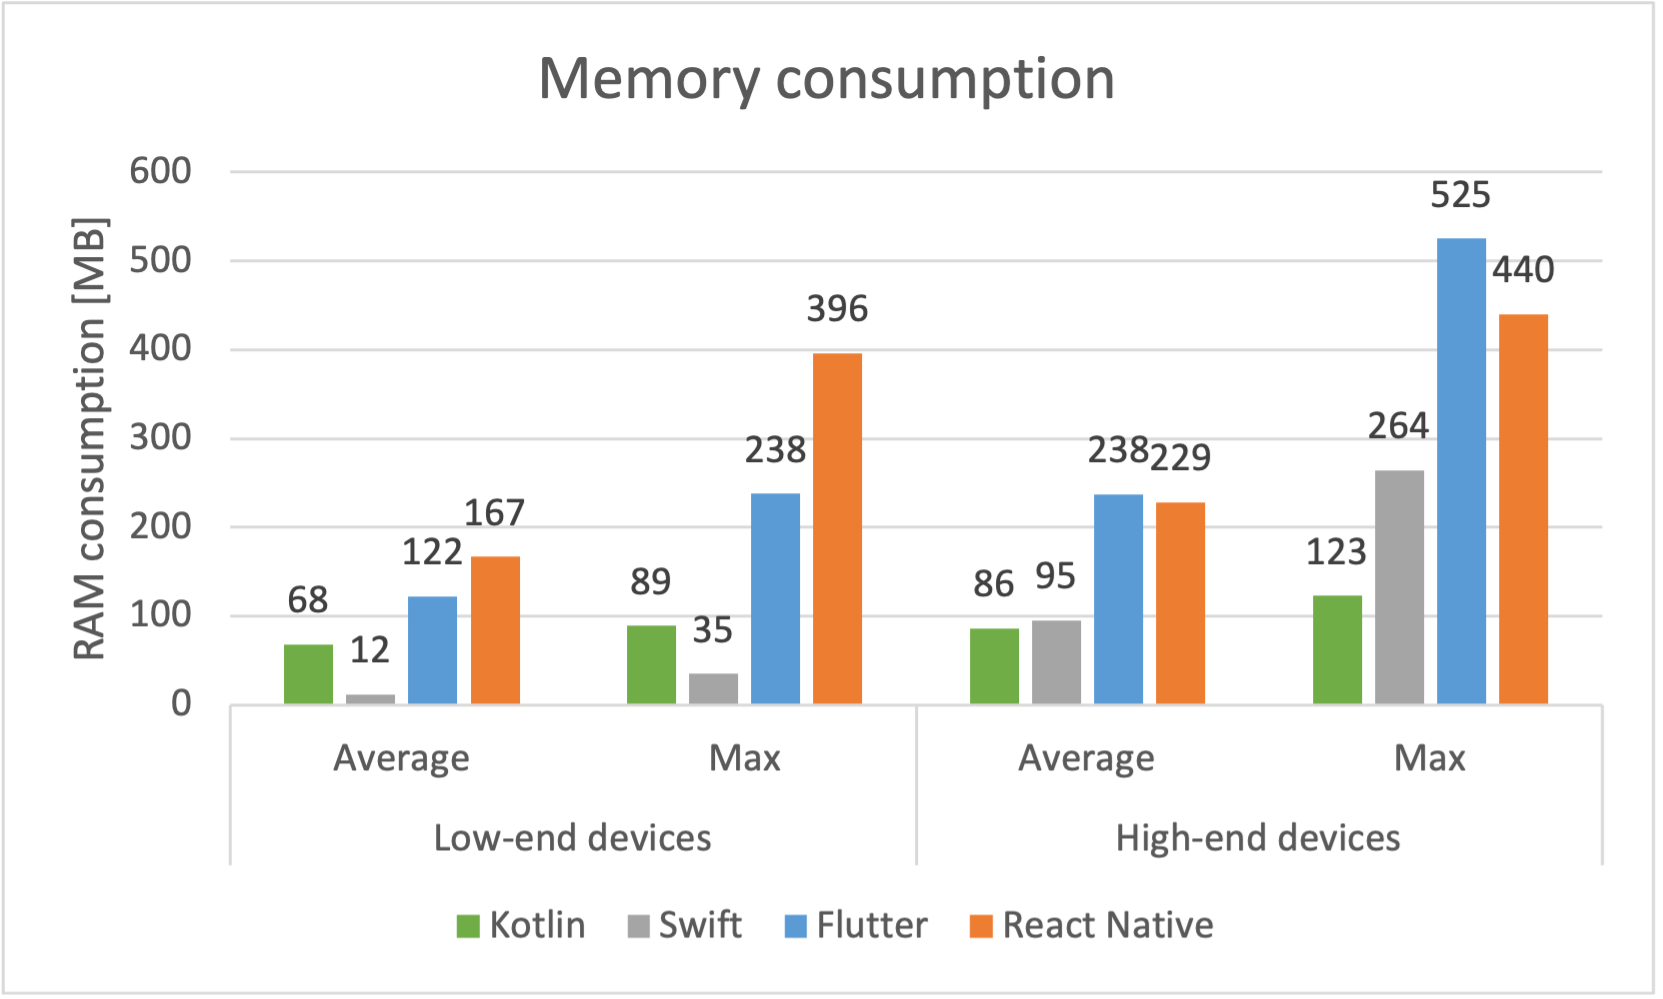
\includegraphics[width=.6\textwidth]{img/scenario3_ram}
    \caption{Research scenario 3: Memory consumption (Source: Own work)}
    \label{fig:s3_ram}
\end{figure}

Figure \ref{fig:s3_ram} shows the comparison of memory consumption among Android and iOS apps developed with Kotlin, Swift, Flutter, and React Native. On low-end devices, Swift apps heavily outperform other technologies; however, on high-end devices, Kotlin apps exhibit the lowest memory usage. Flutter and React Native apps demonstrate similar results. The former utilizes over 30\% less memory on low-end devices but about 4\% more on high-end devices. Analogously, Flutter apps experience smaller spikes on low-end devices and bigger spikes on high-end devices, reaching a maximum of over 500 MB.
